\documentclass[tikz,border=12pt]{standalone}
\usepackage{amsmath}
\usetikzlibrary{arrows.meta,patterns}
\definecolor{meshblue}{RGB}{35,105,170}
\definecolor{material}{RGB}{241,183,112}
\definecolor{history}{RGB}{185,50,65}
\newcommand{\boundary}{(0,-1.4)--(3.6,-1.4)--(5,-.55)--(7,-.55)--(7,.55)--(5,.55)--(3.6,1.4)--(0,1.4)--cycle}
\newcommand{\dies}{
 \fill[pattern=north east lines,pattern color=gray!65] (3.6,1.4)--(5,.55)--(7,.55)--(7,2)--(3.6,2)--cycle;
 \fill[pattern=north east lines,pattern color=gray!65] (3.6,-1.4)--(5,-.55)--(7,-.55)--(7,-2)--(3.6,-2)--cycle;
 \draw[thick] (3.6,1.4)--(5,.55)--(7,.55);
 \draw[thick] (3.6,-1.4)--(5,-.55)--(7,-.55);
}
\begin{document}
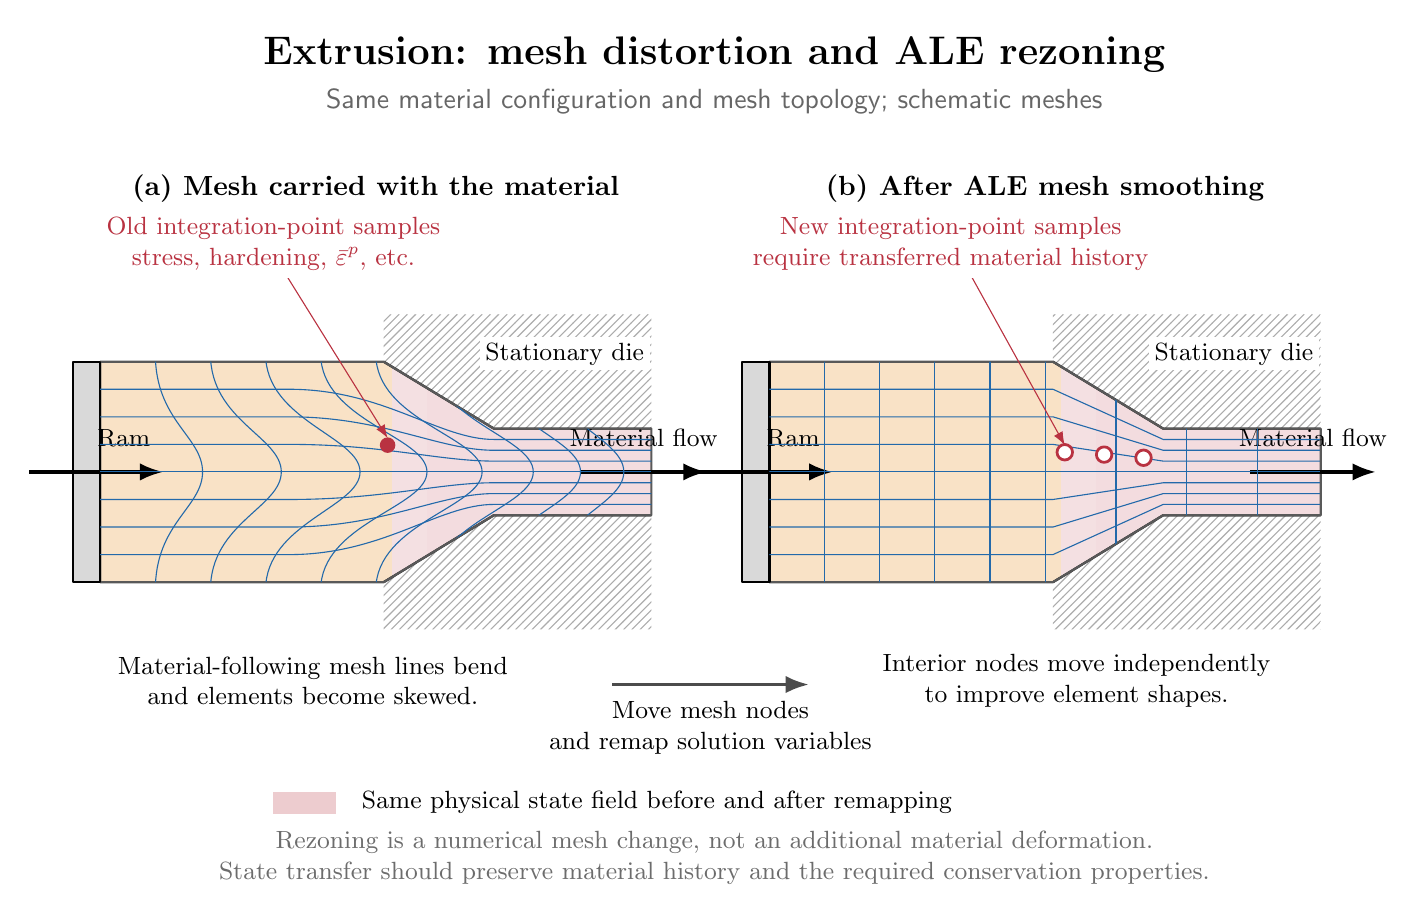
\begin{tikzpicture}[>=Latex,font=\sffamily,line join=round]
\node[font=\Large\bfseries] at (7.8,5.3) {Extrusion: mesh distortion and ALE rezoning};
\node[text=gray!80!black] at (7.8,4.7) {Same material configuration and mesh topology; schematic meshes};
\foreach \dx/\title in {0/{(a) Mesh carried with the material},8.5/{(b) After ALE mesh smoothing}}{
\begin{scope}[shift={(\dx,0)}]
 \node[font=\bfseries] at (3.5,3.6) {\title};
 \fill[material!40] \boundary;
 % A physical state field occupies the same spatial region in both panels.
 \begin{scope}
  \clip \boundary;
  \fill[history!17] (4.15,-2) rectangle (7,2);
  \fill[history!15] (3.7,-2) rectangle (4.15,2);
 \end{scope}
 \dies
 \draw[black!65,thick] \boundary;
 \fill[gray!30] (-.35,-1.4) rectangle (0,1.4);
 \draw[thick] (-.35,-1.4) rectangle (0,1.4);
 \draw[->,very thick] (-.9,0)--(.8,0);
 \node[anchor=south,font=\small] at (.3,.2) {Ram};
 \draw[->,very thick] (6.1,0)--(7.7,0);
 \node[anchor=south,font=\small] at (6.9,.2) {Material flow};
 \node[font=\small,fill=white,inner sep=2pt] at (5.9,1.5) {Stationary die};
\end{scope}}
% Distorted mesh, representing differential material flow near the die.
\begin{scope}
\clip \boundary;
\foreach \f in {-.75,-.5,-.25,0,.25,.5,.75}{
 \draw[meshblue,thin] (0,{1.4*\f})--(2.4,{1.4*\f})
 .. controls (3.6,{1.4*\f}) and (4.3,{.55*\f}) .. (5,{.55*\f})--(7,{.55*\f});
}
\foreach \a/\c in {.7/1.3,1.4/2.3,2.1/3.3,2.8/4.15,3.5/4.85,4.2/5.5,4.9/6.1,5.6/6.65}{
 \draw[meshblue,thin] (\a,-1.5) .. controls (\a,-.65) and (\c,-.45) .. (\c,0)
 .. controls (\c,.45) and (\a,.65) .. (\a,1.5);
}
\end{scope}
% Same 8 transverse and 7 longitudinal interior mesh lines in both panels.
% Each panel has 9 x 8 quadrilateral cells, with unchanged connectivity.
% Smoothed mesh: boundary conforms to the same die and material surface.
\begin{scope}[shift={(8.5,0)}]
\clip \boundary;
\foreach \f in {-.75,-.5,-.25,0,.25,.5,.75}{
 \draw[meshblue,thin] (0,{1.4*\f})--(3.6,{1.4*\f})--(5,{.55*\f})--(7,{.55*\f});
}
\foreach \x in {.7,1.4,2.1,2.8,3.5,4.4,5.3,6.2}{
 \draw[meshblue,thin] (\x,-1.5)--(\x,1.5);
}
\end{scope}
% State samples: not the same integration-point identity after rezoning.
\fill[history] (3.65,.34) circle (2.8pt);
\draw[history,->] (2.3,2.6)--(3.65,.43);
\node[history,align=center,font=\small,fill=white,inner sep=3pt] at (2.2,2.9) {Old integration-point samples\\stress, hardening, $\bar\varepsilon^p$, etc.};
\foreach \x/\y in {12.25/.25,12.75/.22,13.25/.18}{
 \draw[history,fill=white,line width=1pt] (\x,\y) circle (2.8pt);
}
\draw[history,->] (11,2.6)--(12.25,.34);
\node[history,align=center,font=\small,fill=white,inner sep=3pt] at (10.8,2.9) {New integration-point samples\\require transferred material history};
\draw[->,very thick,black!70] (6.5,-2.7)--(9,-2.7);
\node[font=\small,align=center] at (7.75,-3.25) {Move mesh nodes\\and remap solution variables};
\node[align=center,font=\small] at (2.7,-2.65) {Material-following mesh lines bend\\and elements become skewed.};
\node[align=center,font=\small] at (12.4,-2.65) {Interior nodes move independently\\to improve element shapes.};
\draw[history!25,line width=8pt] (2.2,-4.2)--(3,-4.2);
\node[anchor=west,font=\small] at (3.2,-4.2) {Same physical state field before and after remapping};
\node[align=center,font=\small,text=gray!85!black] at (7.8,-4.9) {Rezoning is a numerical mesh change, not an additional material deformation.\\State transfer should preserve material history and the required conservation properties.};
\end{tikzpicture}
\end{document}
